\documentclass[pdf,tikz]{beamer}
\mode<presentation>{}
\usetheme{antibes}
\usepackage[utf8]{inputenc}
\usepackage[ngerman]{babel}

%% präamble
\title{Farben}
\subtitle{Pink fluffy Unicorns oder Black'n'White?}

% pie charts
% math
\usepackage{amsmath}
\usepackage{amssymb}
% tikz
\usepackage{tikz,fourier,ifthen}
\usepackage{pgf}

% custom colors
\usepackage{color}
\definecolor{ppink}{RGB}{255,0,191}
\definecolor{pgreen}{RGB}{0,255,51}
\definecolor{porange}{RGB}{255,206,32}
\definecolor{pgrey}{RGB}{222,221,220}
\definecolor{pdarkblue}{RGB}{30,2,101}


% pie chart
\usetikzlibrary{calc}

\newcommand{\degre}{$^\circ$}


\begin{document}

%-----HEAD-----%
\begin{frame}
	\titlepage
\end{frame}

%-----BODY-----%

\begingroup
\setbeamercolor{background canvas}{bg=ppink}
\begin{frame}
\frametitle{\textcolor{porange}{How NOT to color}}
\begin{itemize}
	\item \textcolor{pgreen}{\Large{Hallo Welt!}}
	\item \textcolor{red}{WICHTIGE} Begriffe sind \textcolor{blue}{farblich} markiert
	\item \textcolor{orange}{Um die \textbf{Konzentration}} der \textcolor{gray}{Leserschaft} zu erhalten, kann man \textbf{viele} \textcolor{green}{Farben} verwenden
\end{itemize}
\end{frame}
\endgroup

\begingroup
\setbeamercolor{background canvas}{bg=pgrey}
\begin{frame}
\frametitle{How to color}
\textcolor{pdarkblue}{Farben sollten sparsam und dezent verwendet werden. Sind wichtige Begriffe vorhanden, so kann man diese \textcolor{red}{markieren}. Jedoch sollte man das nicht zu häufig machen.}
\end{frame}
\endgroup

\begin{frame}
\centering
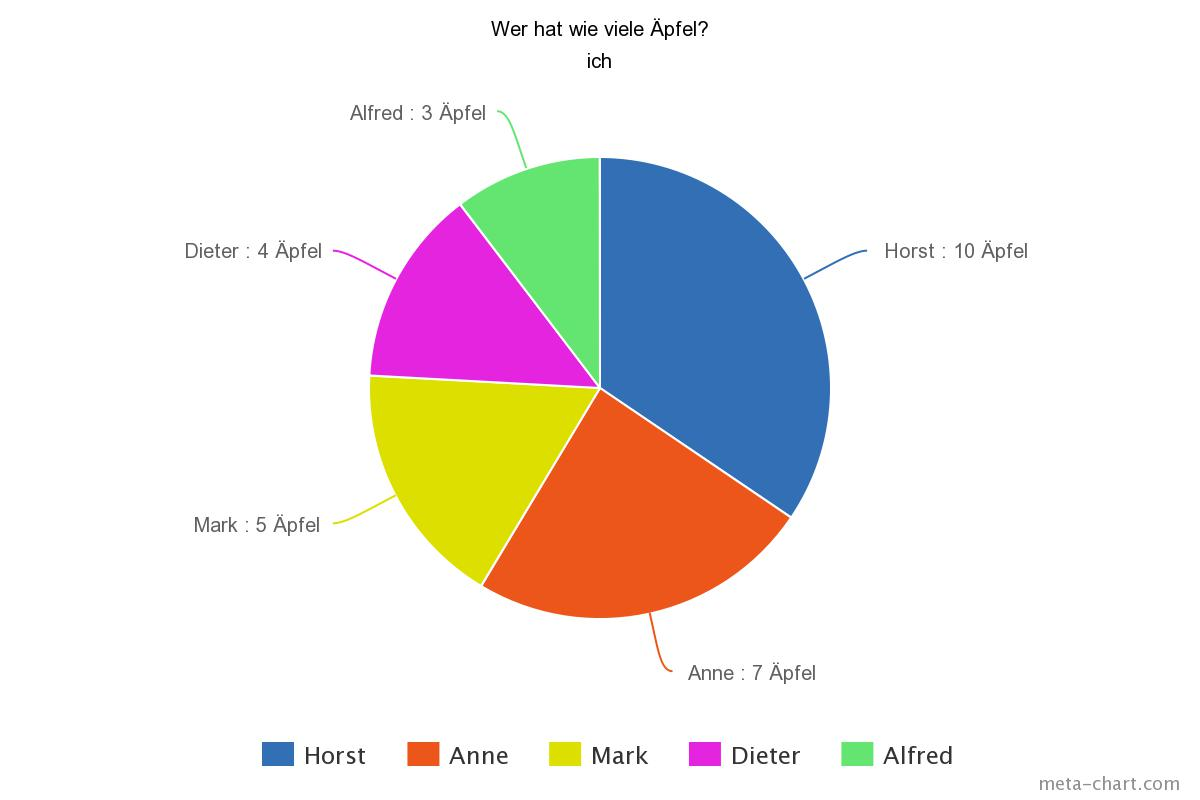
\includegraphics[scale=0.25]{apfelchart}
\end{frame}


\end{document}